\documentclass[11pt,a4paper]{article}
\usepackage{fontspec}
\setmainfont{TeX Gyre Termes}
\setmonofont{Latin Modern Mono}[Scale=0.95]
\usepackage[margin=2.6cm,top=2.8cm,bottom=2.8cm]{geometry}
\usepackage{graphicx,booktabs,amsmath,xcolor,fancyhdr,caption,titlesec,microtype,enumitem,tabularx}
\usepackage{xurl}
\usepackage[hidelinks,pdftitle={Between Sustainability and Competitiveness: The Atalanta Model},pdfauthor={Ettore Mancuso},pdfsubject={Financial statement analysis of Atalanta B.C., 2016 to 2024/25},pdfkeywords={football finance, financial statement analysis, Serie A, private equity}]{hyperref}
\usepackage{float}
\usepackage{placeins}
\usepackage[round,authoryear]{natbib}

\captionsetup{font={small,it},labelfont={small,it},justification=centering}
\titleformat{\section}{\large\bfseries}{\thesection.}{0.5em}{}
\titleformat{\subsection}{\normalsize\bfseries}{\thesubsection}{0.5em}{}
\titlespacing*{\section}{0pt}{14pt}{6pt}
\titlespacing*{\subsection}{0pt}{10pt}{4pt}
\setlength{\parskip}{5pt}\setlength{\parindent}{0pt}\setlength{\emergencystretch}{2em}
\newcolumntype{L}{>{\raggedright\arraybackslash}X}
\newcolumntype{P}[1]{>{\raggedright\arraybackslash}p{#1}}

\pagestyle{fancy}\fancyhf{}
\fancyhead[L]{\small\itshape The Atalanta Model}
\fancyhead[R]{\small\itshape Ettore Mancuso}
\fancyfoot[C]{\small\thepage}
\renewcommand{\headrulewidth}{0.4pt}\renewcommand{\footrulewidth}{0.4pt}

\begin{document}
\thispagestyle{empty}
\begin{center}
{\LARGE\bfseries Between Sustainability and Competitiveness:\\[4pt] The Atalanta Model}\\[10pt]
{\large\itshape Ten years of financial statements of a Serie A club\\ that keeps closing in profit, 2016 to 2024/25}\\[22pt]
{\large Ettore Mancuso}\\[1pt]
\href{mailto:ettoremancuso6@gmail.com}{ettoremancuso6@gmail.com}\\[1pt]
October 2026
\end{center}
\vspace{16pt}

\section*{Abstract}
Between 2016 and 2024/25, the nine seasons with Gian Piero Gasperini as coach, Atalanta closed ten consecutive financial years in profit, EUR~230.5m in total, while Serie A as a whole kept losing money. My thesis is that selling players is Atalanta's core business, not an occasional source of income. The club buys young players cheaply, plays them, sells them near their peak and reinvests the proceeds. Using the published accounts, I show that gains on player disposals added up to EUR~534m over the period, 27.5\% of revenue. In 2024/25, the club's best year, reported EBIT was EUR~59.1m; without player trading it would have been about EUR~−62m. I then look at how a gain on disposal is booked under Italian GAAP, at cash and equity, at a comparison with Bayern Munich, and at the 2022 entry of Stephen Pagliuca's group, which I read as a private equity deal (implied gross MOIC of 29 to 36 times for the Percassi family over twelve years), and model the buyers' side as a holding-company LBO: with 83\% debt and PIK interest, the club has to be worth about 2.1 times its revenue by 2027 for the American investors just to get their money back. The first half of 2025/26, after Gasperini left, closed with EUR~27.1m of profit, so the model did not depend on him alone. It is profitable, but it runs on a single engine, and that is its main risk. All data and code are public.

\medskip
\textbf{Keywords:} football finance, financial statement analysis, player trading, intangible assets, OIC~24, private equity, leveraged buyout, PIK debt, Serie A

\textbf{JEL classification:} G32, G34, M41, Z23

\section{Introduction}
Italian football is not a good business. In 2023/24 Serie A clubs reported an aggregate net loss of EUR~369m, with personnel costs equal to 52\% of revenue \citep{cef_seriea2324}. In 2024/25 only seven of the twenty clubs closed in profit, and in the two seasons hit hardest by Covid there were two \citep{cef_seriea2425}. Atalanta, a club from a city of about 120,000 people, was one of the two in the Covid years, and in 2024/25 it reported the highest net profit in the league, EUR~37.9m, ahead of an Inter side that played a Champions League final and the Club World Cup with roughly three times its revenue (Figure~\ref{fig:league}).

The questions I try to answer are:
\begin{enumerate}[leftmargin=1.5em,itemsep=2pt]
\item How does Atalanta make money, and how much of its profit comes from selling players?
\item What does the club look like once gains on disposals are separated from recurring revenue?
\item How solid is the balance sheet, and what did the 2022 change of ownership mean for the people who built the club?
\item Does the model survive the departure of the coach who made it famous, and where could it break?
\end{enumerate}

Section~2 describes the business model and Section~3 the data. Section~4 goes through ten years of results, Section~5 the 2024/25 income statement and the profit bridge, Section~6 the accounting of a gain on disposal. Section~7 covers cash and equity, Section~8 the comparison with Bayern Munich, Section~9 the Pagliuca deal and Section~10 the first season after Gasperini. Section~11 lists the risks and Section~12 concludes.

\begin{figure}[htbp]\centering
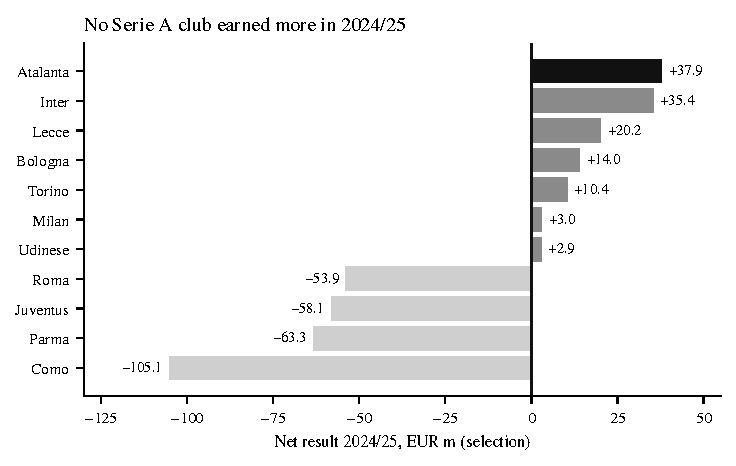
\includegraphics{../figures/fig4_serie_a_2024_25.pdf}
\caption{Net result 2024/25 of a selection of Serie A clubs, EUR million. Source: \citet{cef_seriea2425}.}\label{fig:league}
\end{figure}

\section{The business model}
The model is a cycle that repeats. Each sale pays for the next round.
\begin{enumerate}[leftmargin=1.5em,itemsep=2pt]
\item \textbf{Scouting.} Players come from the Zingonia academy or are bought young, often abroad, at a low price.
\item \textbf{Development.} Gasperini's system gives new players minutes and visibility.
\item \textbf{Competition.} European football brings UEFA prize money: EUR~67.1m from the Champions League in 2024/25.
\item \textbf{Sale.} The player is sold close to the peak of his value.
\item \textbf{Reinvestment.} The proceeds go back into the squad, the stadium and the training centre.
\end{enumerate}

Rasmus Højlund is a good example. He arrived from Sturm Graz in summer 2022 for about EUR~17m and left for Manchester United a year later for more than EUR~70m, a gain of EUR~53.2m \citep{cef_mercato2023}. With that money Atalanta signed Scamacca, De~Ketelaere, Touré, Bakker and then Hien, a large part of the team that won the Europa League in 2024.

Four conditions hold the cycle together. The club owns its stadium, bought from the city in 2017 for EUR~8.6m and rebuilt for about EUR~100m, partly with a dedicated EUR~40m loan from Credito Sportivo and Intesa Sanpaolo \citep{ilgiorno_stadio,italpress_stadio}. Ownership has been stable: the Percassi family since 2010, joined in 2022 by Pagliuca's group. Wages are under control, at 39.7\% of revenue in 2024/25 against the Serie A average of 52\%. And the training centre keeps receiving money, with another EUR~20m for the Zingonia expansion funded by the 2025 capital increase.

\section{Data}
All figures come from Atalanta B.C.'s filed financial statements, as reported by Calcio e Finanza \citep{cef_1620,cef_2021,cef_2324,cef_2425,cef_h1}, with QuiFinanza for the gains on disposals of the earlier years \citep{qf_plusvalenze}. I collected them by hand into five CSV files, each with a source column (Table~\ref{tab:data}). Two details matter for reading the series.

First, the calendar. Until 2021 the financial year ended on 31 December. To align with the football season the club then filed a six-month period, January to June 2022, and since then the year runs from July to June. The six-month period is included in the totals and flagged in the charts. Second, restatements. For 2022/23 and 2023/24 some sources report a net profit of EUR~3.8m and 9.8m. I use the figures restated in the following year's accounts, EUR~5.6m and 11.8m, which are the most recent version. Gains on the 2026 sales are press estimates and are marked as such. MOIC, IRR, multiples, the profit bridge and the ratios are my own calculations.

\begin{table}[H]\centering\small
\caption{Data files in the repository.}\label{tab:data}
\begin{tabularx}{\textwidth}{p{5.6cm}L}
\toprule
File & Content \\
\midrule
\texttt{financials\_by\_period.csv} & Revenue, gains on player disposals and net profit, 2016 to 2024/25 \\
\texttt{pnl\_2024\_25.csv} & Income statement 2024/25 and 2023/24 \\
\texttt{equity.csv} & Shareholders' equity, December 2019 to December 2025 \\
\texttt{serie\_a\_net\_results\_2024\_25.csv} & Net result of a selection of Serie A clubs \\
\texttt{top\_player\_sales.csv} & The ten largest gains on disposal in the club's history \\
\bottomrule
\end{tabularx}
\end{table}

\section{Ten years of results}
Revenue went from EUR~83.1m in 2016 to EUR~320.8m in 2024/25, almost four times as much, a compound growth rate of about 17\% a year. Two things drove it: European competitions and gains on disposals, which were between 16\% and 37\% of revenue every year and 27.5\% on average (Figure~\ref{fig:rev}).

\begin{figure}[htbp]\centering
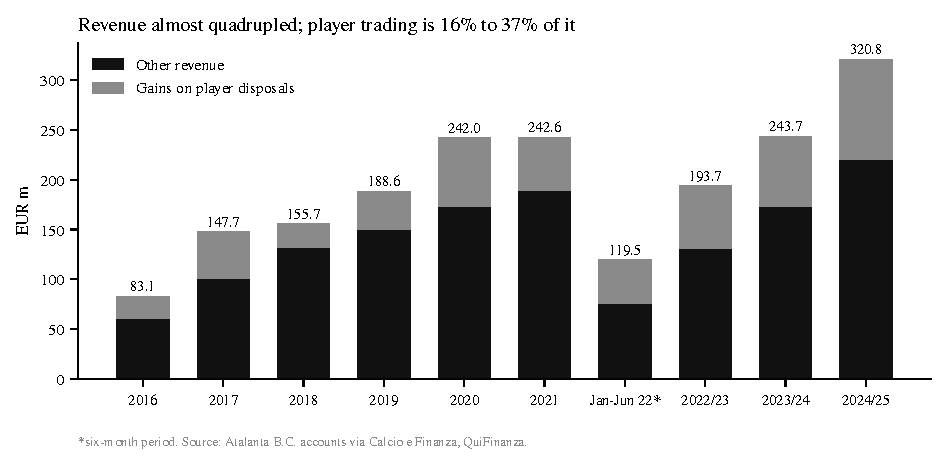
\includegraphics[width=\textwidth]{../figures/fig1_revenue_split.pdf}
\caption{Revenue split between gains on player disposals and other revenue, EUR million.}\label{fig:rev}
\end{figure}

The year that says the most is 2022/23, the only one without European football: revenue fell to EUR~193.7m. The 2024/25 season, Gasperini's last, is the record, with EUR~67.1m from the new Champions League format and EUR~100.9m of gains on disposals.

Net profit was positive every year (Figure~\ref{fig:profit}). The peak, EUR~51.7m in 2020, coincides with the Champions League quarter-final against Paris Saint-Germain and the sale of Kulusevski to Juventus. Across 2020 and 2021, in the middle of the pandemic, the club earned EUR~86.8m while almost all of Serie A was in the red. The low point is 2022/23, EUR~5.6m: without Europe, the profit was there only because of EUR~63.2m of gains on disposals.

\begin{figure}[htbp]\centering
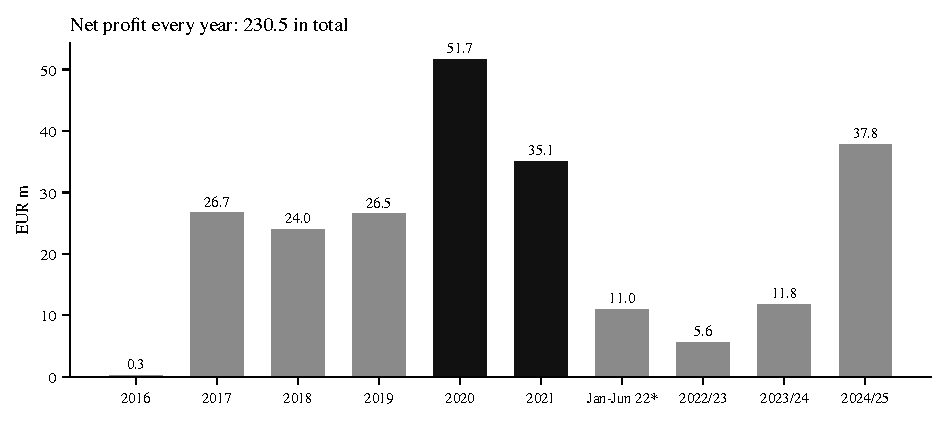
\includegraphics[width=\textwidth]{../figures/fig2_net_profit.pdf}
\caption{Net profit, EUR million. The two Covid years, 2020 and 2021, in black. 2022/23 and 2023/24 as restated in the following year's accounts.}\label{fig:profit}
\end{figure}

\section{The 2024/25 income statement}
Gasperini's last season is also the richest in the club's history: EUR~320.8m of revenue, EUR~261.7m of costs and EUR~37.8m of net profit (Table~\ref{tab:pnl}).

\begin{table}[H]\centering\small
\caption{Income statement, EUR million. Source: \citet{cef_2425}.}\label{tab:pnl}
\begin{tabular}{lrr}
\toprule
 & 2024/25 & 2023/24 \\
\midrule
TV and media rights (of which UEFA 67.1) & 138.6 & 107.5 \\
Player trading (of which gains on disposals 100.9 and 71.0) & 121.6 & 83.7 \\
Sponsorship, commercial and royalties & 37.7 & 32.3 \\
Gate receipts & 15.1 & 11.6 \\
Other revenue & 7.8 & 8.7 \\
\textbf{Total revenue} & \textbf{320.8} & \textbf{243.7} \\
\midrule
Personnel & 127.4 & 120.1 \\
Depreciation and amortisation (of which players 71.2 and 48.9) & 76.7 & 54.0 \\
Other operating costs & 31.2 & 26.3 \\
Services & 26.5 & 23.4 \\
\textbf{Total costs} & \textbf{261.7} & \textbf{223.7} \\
\midrule
\textbf{Net profit} & \textbf{37.8} & \textbf{11.8} \\
\bottomrule
\end{tabular}
\end{table}

In the Italian statutory format gains on disposals sit inside the value of production, next to TV money and tickets. That is why a club's ``turnover'' has to be taken apart: the EUR~121.6m from player trading will not come back every year the way TV rights do. I therefore rebuilt the result starting from structural revenue only, defined as TV, sponsorship, gate receipts and other revenue (Figure~\ref{fig:bridge}).

\begin{figure}[htbp]\centering
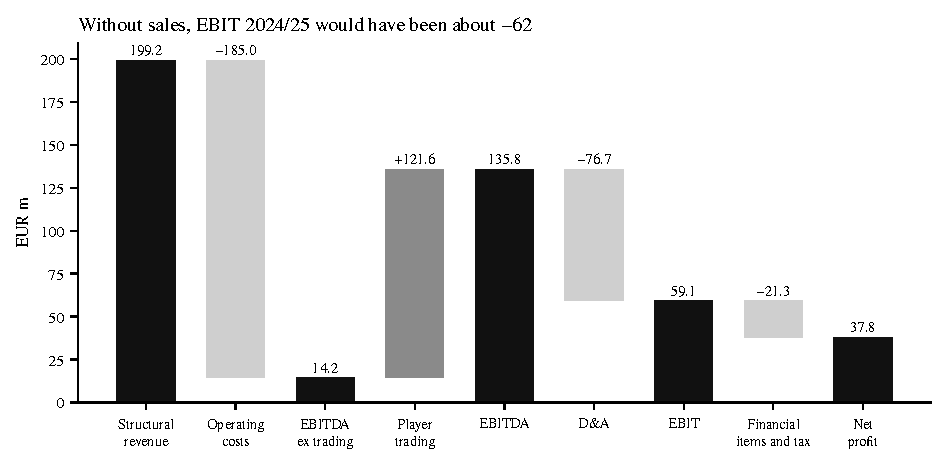
\includegraphics[width=\textwidth]{../figures/fig3_profit_bridge_2024_25.pdf}
\caption{From structural revenue to net profit, 2024/25, EUR million. Operating costs are total costs minus depreciation and amortisation. My elaboration on the accounts at 30 June 2025.}\label{fig:bridge}
\end{figure}

Without player sales, EBITDA is only EUR~14.2m. After depreciation and amortisation, which stay because the squad has to be bought whether or not anyone is sold, EBIT would be about EUR~−62m. Sales cover that gap and produce the profit. The EBITDA of EUR~135.8m matches the figure Calcio e Finanza uses in its comparison with Bayern \citep{cef_bayern}, so the numbers reconcile. The same calculation for 2023/24 gives a similar result, about EUR~−64m. For a club that lives on sales, the right question is not whether there is a profit but whether there will be more players to develop and sell.

\section{How a gain on disposal is booked}
A gain on disposal (\textit{plusvalenza}) is the difference between the sale price of a player and the net book value of his registration. To see why Atalanta generates so many of them, it helps to follow a registration through its life on the balance sheet.

\begin{enumerate}[leftmargin=1.5em,itemsep=2pt]
\item \textbf{Recognition.} The registration is an intangible asset (rights to the player's services, OIC~24), recorded at purchase cost plus ancillary costs such as agents' fees.
\item \textbf{Amortisation.} It is amortised on a straight line over the length of the contract. If the player renews, the residual value is spread over the new term.
\item \textbf{Sale.} The gain is price minus net book value. It enters the value of production, so it raises reported revenue.
\item \textbf{Academy players.} Youth sector costs are expensed year by year, so a player who grew up at the club reaches the sale with a book value close to zero, and almost the whole price becomes gain.
\end{enumerate}

\begin{table}[H]\centering\small
\caption{The Koopmeiners case, EUR million. Sources: \citet{cm_koop}; \citet{cef_2324,cef_2425}.}\label{tab:koop}
\begin{tabular}{lr}
\toprule
Bought from AZ Alkmaar (2021) & 14.0 \\
Net book value at 30 June 2023 & 8.3 \\
Net book value at 30 June 2024, after renewal to 2027 & about 6.2 \\
Sale price to Juventus (2024) & 51.3 \\
\textbf{Gain recognised in 2024/25} & \textbf{44.5} \\
\bottomrule
\end{tabular}
\end{table}

The price exceeds the book value by about EUR~45m, and the accounts show EUR~44.5m. The difference comes from ancillary costs and contract clauses, such as the 10\% of the amount above EUR~14m owed to AZ. The exact reconciliation is in the notes to the accounts. The extreme case is Marco Palestra: an academy player with a book value of zero at 30 June 2025, sold to Chelsea in June 2026 for EUR~55 to 57m plus bonuses, for a gain of at least EUR~55m, the largest in the club's history \citep{cef_palestra}.

\section{Cash and the balance sheet}
Profit is not cash. A gain is recognised when the sale closes, but the price is often paid in instalments. I therefore also looked at cash flows and at the balance sheet (Table~\ref{tab:cash}).

\begin{table}[H]\centering\small
\caption{Cash and balance sheet indicators. Sources: \citet{cef_2425,cef_h1,cef_mercato2023,italpress_stadio}.}\label{tab:cash}
\begin{tabularx}{\textwidth}{P{4.3cm}P{3.3cm}L}
\toprule
Indicator & Value & How to read it \\
\midrule
Self-financing 2024/25 & EUR~114.5m & Net profit 37.8 plus D\&A 76.7, to be read together with player purchases \\
Transfer balance, summer 2023 & +EUR~66.1m & Sales 131.8 against purchases 65.7 (official figures) \\
Payables / receivables with clubs, 31 Dec 2025 & EUR~143m / 135m & Purchases paid in instalments are almost fully covered by sales paid in instalments \\
Cash & EUR~43.7m to 93.0m & June to December 2025, after the sales of Retegui and Ruggeri \\
Financial debt / equity & 0.22 & EUR~54.8m against EUR~248.2m, June 2025 \\
Stadium financing & EUR~40m & Dedicated loan: long-term investment, long-term debt \\
\bottomrule
\end{tabularx}
\end{table}

Between the end of 2019 and June 2025 equity grew by EUR~170.4m. Over the same period the club earned EUR~153.0m, so about 90\% of the growth came from retained profits (Figure~\ref{fig:equity}). The rest are other equity movements; in 2025 there was also a EUR~72m capital increase at the holding, partly used for Zingonia. For some dates the sources give slightly different values (for example EUR~190.9m or 196.3m at June 2024) because later accounts restate them. The conclusion does not change.

\begin{figure}[htbp]\centering
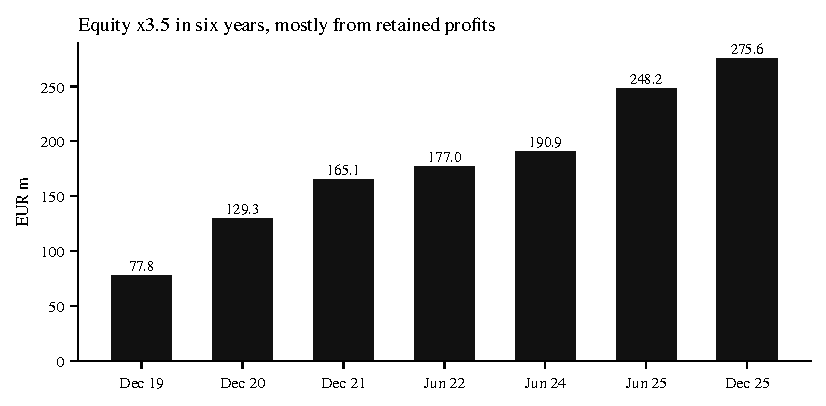
\includegraphics{../figures/fig5_equity.pdf}
\caption{Shareholders' equity, EUR million. June 2023 is left out because the sources disagree.}\label{fig:equity}
\end{figure}

An insurer would recognise the logic: a capital buffer built from recurring profits is the first protection in bad years. Atalanta has the same kind of solidity, with one difference. Its profits depend largely on sales.

\section{Efficiency: a comparison with Bayern Munich}
Bayern takes in three times as much, yet in 2024/25 Atalanta closed with a higher net profit and an EBIT margin almost five times larger (Table~\ref{tab:bayern}). I chose Bayern because it is Europe's reference for a sustainable club, in profit for 33 years, and because the two teams met in the Champions League round of 16 in March 2026.

\begin{table}[H]\centering\small
\caption{Atalanta and Bayern Munich, 2024/25, EUR million. Source: \citet{cef_bayern}.}\label{tab:bayern}
\begin{tabular}{lrr}
\toprule
 & Atalanta & Bayern Munich \\
\midrule
Total revenue & 320.8 & 978.3 \\
\quad of which player trading & 121.6 & 117.7 \\
Personnel costs & 127.4 & 443.5 \\
Personnel / revenue & 39.7\% & 45.3\% \\
EBITDA & 135.8 & 187.8 \\
EBIT & 59.1 & 38.5 \\
EBIT margin & 18.4\% & 3.9\% \\
Net profit & 37.9 & 27.1 \\
Equity & 248.2 & 585.5 \\
Financial debt & 54.8 & 0 \\
\bottomrule
\end{tabular}
\end{table}

What surprised me most is that the two clubs earn almost the same amount from player trading. The whole difference is in structural revenue, EUR~199m against EUR~861m. It also changes how the wage figure reads. Wages are 39.7\% of total revenue, well below the Serie A average of 52\%. Measured on structural revenue alone, without sales, they rise to 64\%. The wage discipline is real, but sustainability still depends on selling.

\section{The Pagliuca deal, read as private equity}
In February 2022 a group of American investors led by Stephen Pagliuca, co-chairman of Bain Capital and co-owner of the Boston Celtics, bought 55\% of the Percassi family's holding company. This is the part of the work I find most interesting, and I rebuilt it as if it were a deal (Table~\ref{tab:deal}). The debt used to pay for the acquisition sits in a vehicle above the club, not in the club itself, and Pagliuca said so explicitly in 2022: the financing weighs on the shareholders, not on Atalanta \citep{cef_pagliuca}.

\begin{table}[H]\centering\small
\caption{Simplified term sheet. Sources: \citet{bebeez,investireoggi,cef_pegno,cef_aucap,ilfoglio}.}\label{tab:deal}
\begin{tabularx}{\textwidth}{P{3.6cm}L}
\toprule
Item & Detail \\
\midrule
Stake acquired & 55\% of the holding La Dea H, about 47\% of the club indirectly \\
Valuation & Enterprise value of about EUR~400m; press reports of EUR~440 to 500m for 100\% \\
Acquisition debt & EUR~152.5m bond issued by Athena S.p.A., PIK toggle 8\% / 8.75\%, maturing April 2027 \\
Vendor loan & EUR~23m from the Percassi family, secured on the majority stake \\
Lenders & Vehicles linked to Carlyle and Ares, with a pledge on the shares \\
Co-investor & Arctos Sports Partners, minority stake of USD~36m \\
Follow-on & EUR~72m capital increase (January 2025): EUR~67m from the American investors, EUR~5m from the Percassi family; US share up to 62\% \\
Governance & Antonio and Luca Percassi as chairman and CEO, Pagliuca as co-chairman \\
\bottomrule
\end{tabularx}
\end{table}

For the people who built it, the model paid off. The Percassi family took over the club in 2010 for about EUR~14m; in 2022 the deal valued it at EUR~400 to 500m (Table~\ref{tab:multiples}).

\begin{table}[H]\centering\small
\caption{Implied returns and multiples. My calculations on \citet{ilfoglio} and \citet{cef_2021}.}\label{tab:multiples}
\begin{tabular}{lr}
\toprule
MOIC, 2010 to 2022 & 29 to 36x \\
Gross IRR over 12 years & 32 to 35\% a year \\
Price / revenue 2021 (EUR~242.6m) & 1.8 to 2.1x \\
Price / equity 2021 (EUR~165.1m) & 2.7 to 3.0x \\
Price / earnings 2021 (EUR~35.1m) & 12.5 to 14.2x \\
\bottomrule
\end{tabular}
\end{table}

MOIC and IRR are gross: they ignore the capital put back into the club (stadium, Zingonia) and the profits left in it. A P/E of about 13 is the multiple of a company that makes profits, which is rare for a football club; clubs are usually priced on revenue multiples.

The open question is the bond. It is structurally subordinated: to repay it, the holding needs dividends from the club, a refinancing or an exit. It matures in April 2027, six months from now, and I found no public news of a refinancing. For an investor, it is the next thing to watch.

\subsection{An LBO view of the American investors' returns}
The Percassi family's return is the easy half of the story. The other half is the buyer's. The American investors did not buy the club directly: their vehicle, Athena S.p.A., bought a stake in the holding and paid mostly with borrowed money. That is a holding-company leveraged buyout, and it can be modelled like one. I rebuilt it in a small Python module (\texttt{src/pe\_returns.py}) using the public figures in Table~\ref{tab:deal} and four assumptions, all of which can be changed:
\begin{enumerate}[leftmargin=1.5em,itemsep=2pt]
\item 100\% of the club valued at EUR~450m at entry, the middle of the press range, so the 47\% look-through stake cost about EUR~211.5m;
\item bond interest always paid in kind at 8.75\%, which is the natural choice when the club pays no dividends and the worst case for the equity;
\item the vendor loan repaid at face value, and the EUR~67m US share of the 2025 capital increase counted as extra equity;
\item exit value of the club expressed as a multiple of 2024/25 revenue (EUR~320.8m). The 2022 price was about 1.85 times 2021 revenue.
\end{enumerate}

\begin{table}[H]\centering\small
\caption{Sources and uses at entry, EUR million. My reconstruction; the equity cheque is the balancing item and includes Arctos's minority ticket.}\label{tab:su}
\begin{tabular}{lrr}
\toprule
 & EUR m & \% of price \\
\midrule
\textit{Uses} & & \\
\quad 47\% look-through stake in the club & 211.5 & 100\% \\
\textit{Sources} & & \\
\quad PIK toggle bond (Athena S.p.A.) & 152.5 & 72\% \\
\quad Vendor loan (Percassi family) & 23.0 & 11\% \\
\quad Equity (US investors and Arctos) & 36.0 & 17\% \\
\bottomrule
\end{tabular}
\end{table}

Table~\ref{tab:su} shows why the deal deserves attention. Debt covers 83\% of the price, a loan-to-value that would be aggressive for any buyout and is unusual for a football club. With interest paid in kind, the bond grows by 8.75\% a year whatever the club does: by the April 2027 maturity the holding owes about EUR~256.5m, against EUR~175.5m at entry (Figure~\ref{fig:holdco}).

\begin{figure}[htbp]\centering
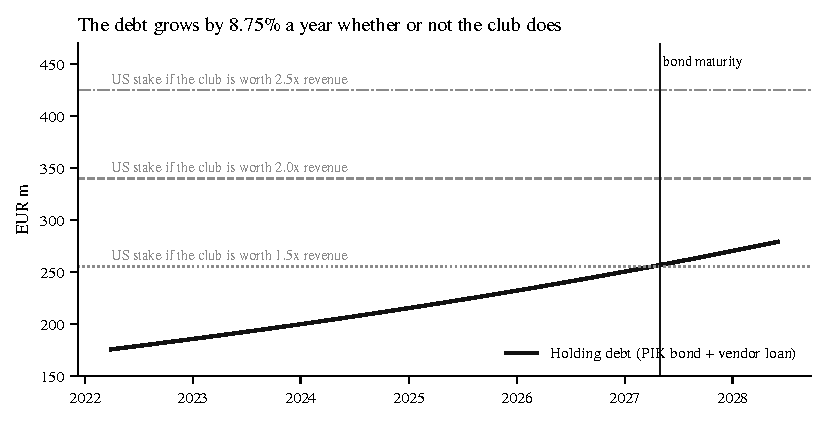
\includegraphics{../figures/fig8_holdco_debt.pdf}
\caption{Debt at the holding against the value of the US investors' 53\% look-through stake for three club valuations, EUR million. My model; interest assumed paid in kind.}\label{fig:holdco}
\end{figure}

From there the arithmetic is simple. At maturity the club has to be worth about EUR~484m (1.5 times 2024/25 revenue) just for the stake to cover the debt. For the investors to get their money back, EUR~103m in total, it has to be worth about EUR~679m, 2.1 times revenue. If it were sold at the same multiple paid in 2022, 1.85 times, the equity would get back 0.57 times its money, an IRR of about −17\% a year. Revenue grew a lot after 2022, but the leverage and the PIK interest grew faster. Figure~\ref{fig:pe} shows the full grid of outcomes. The same model is also built as a spreadsheet, \texttt{model/atalanta\_lbo.xlsx}, laid out the way an LBO is usually presented in banking: transaction assumptions, sources and uses, an operating model of the club, the debt schedule, returns, breakeven values, four 5×5 sensitivity tables with the base case in the centre, and a block of checks that must all read zero (Figures~\ref{fig:xlsx} to~\ref{fig:xlsx3}). Every number is a formula, so changing the entry value, the PIK rate, the revenue growth or the exit multiple updates the whole sheet. It gives the same numbers as the Python module.

\begin{figure}[htbp]\centering
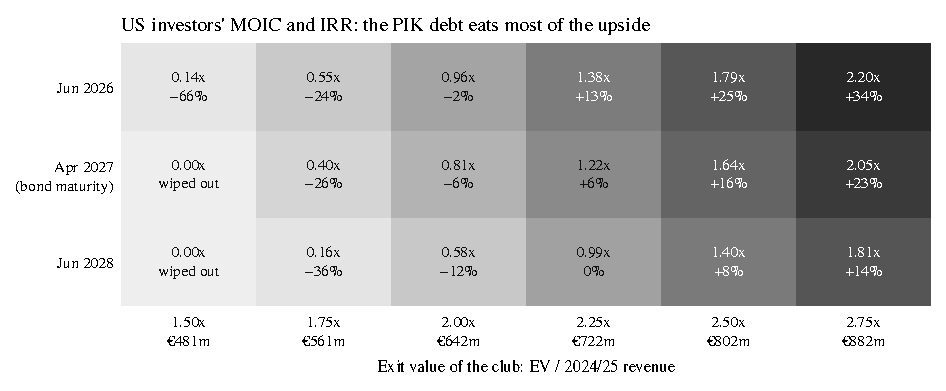
\includegraphics[width=\textwidth]{../figures/fig7_pe_returns_sensitivity.pdf}
\caption{MOIC and IRR of the US equity by exit date and exit valuation. Rows: exit date; columns: club value as a multiple of 2024/25 revenue. My model on public figures.}\label{fig:pe}
\end{figure}

Two things move the result most. The first is the entry price: at EUR~400m for 100\% the equity cheque falls to EUR~12.5m and the loan-to-value rises to 93\%; at EUR~500m it is EUR~59.5m and 75\%. The second is time. Every year of waiting adds interest, so the same exit value is worth less to the equity in 2028 than in 2026. This is the classic trade-off of a PIK structure: it saves cash today but makes the exit date and the exit multiple decide almost everything. It also explains why the April 2027 maturity matters. A refinancing, a dividend recapitalisation at the club or a sale of part of the stake are the natural ways out, and each would change the risk for the club's other shareholders.

\begin{figure}[p]\centering
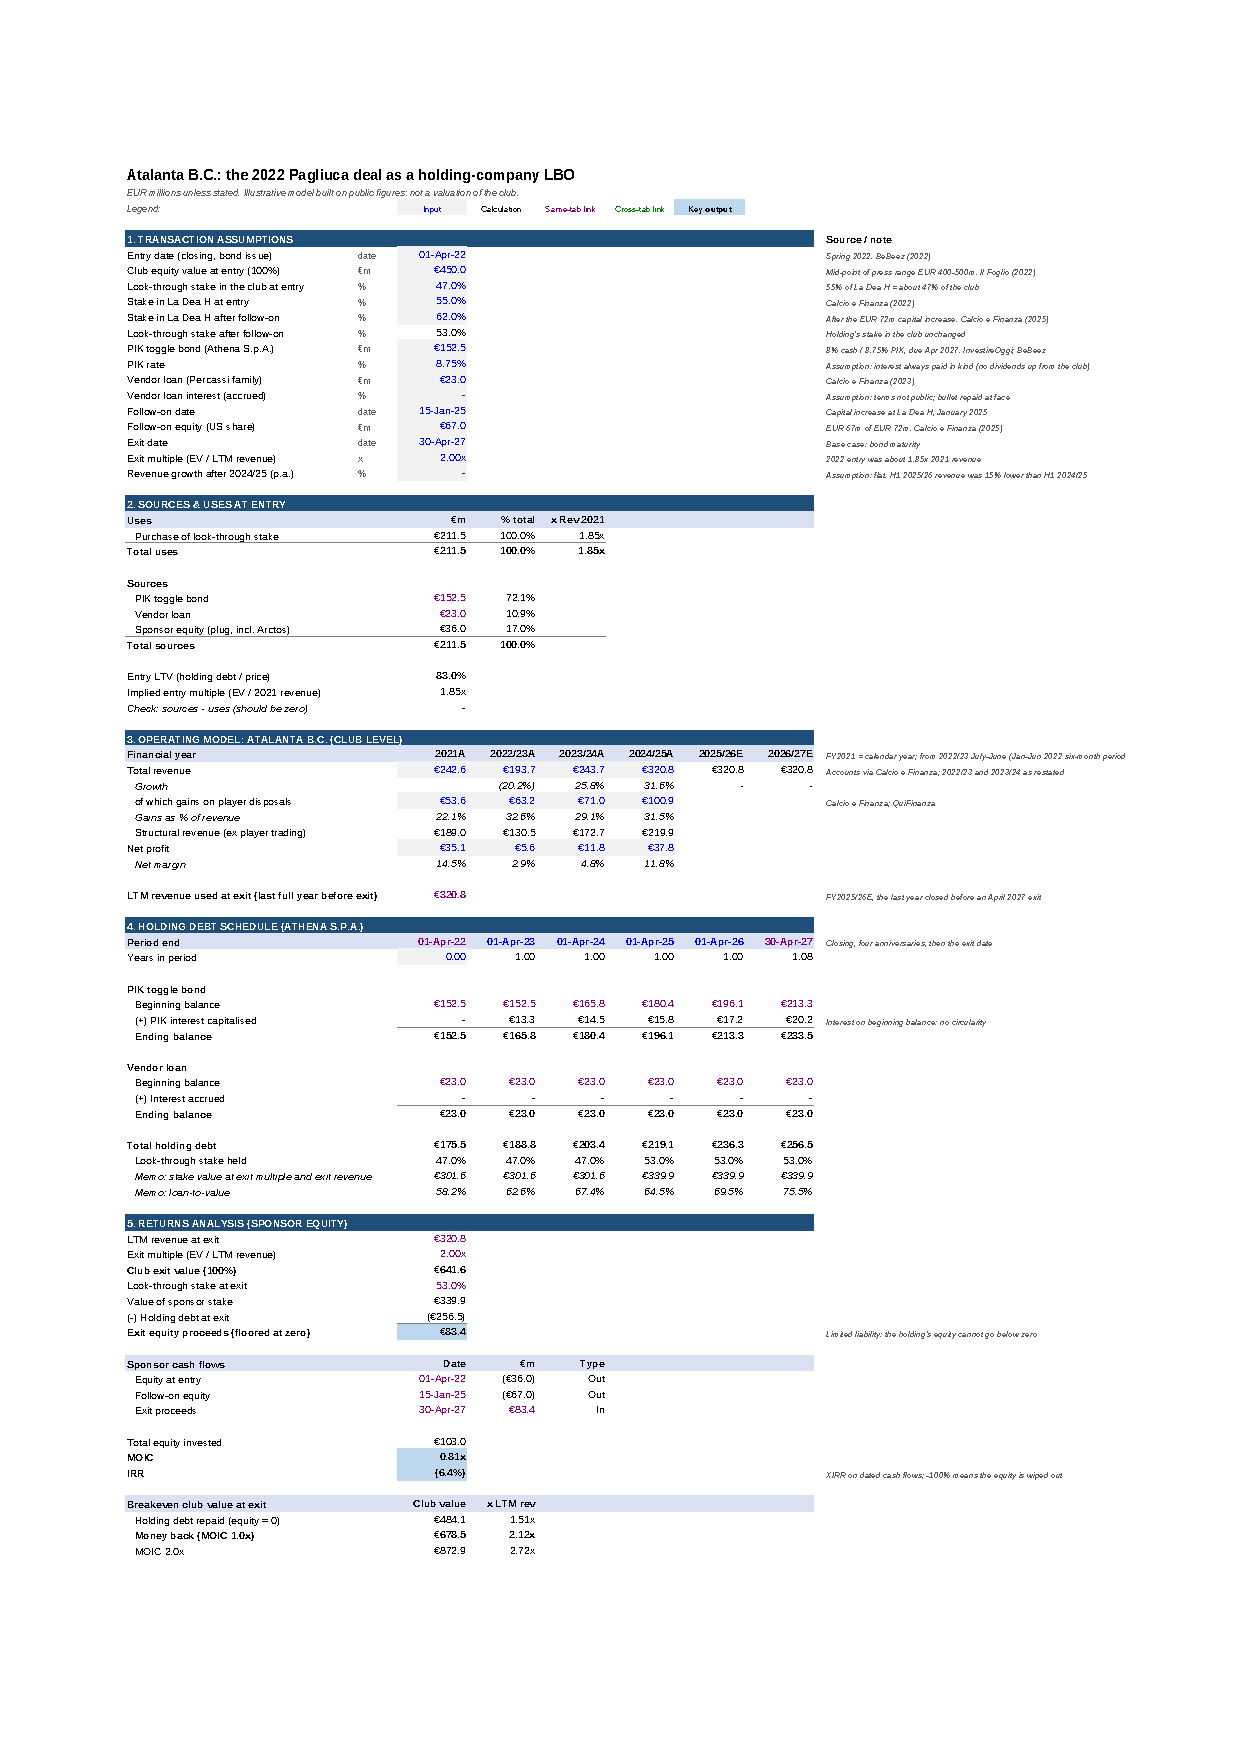
\includegraphics[width=\textwidth,trim=56 406 203 76,clip,page=1]{../model/atalanta_lbo_print.pdf}
\caption{The LBO model in Excel (\texttt{model/atalanta\_lbo.xlsx}), part 1: transaction assumptions, sources and uses, and the club's operating model. Blue font marks inputs, black calculations, purple links within the sheet and green links to another sheet; shaded cells are key outputs. The workbook also lists the source of every input.}\label{fig:xlsx}
\end{figure}

\begin{figure}[p]\centering
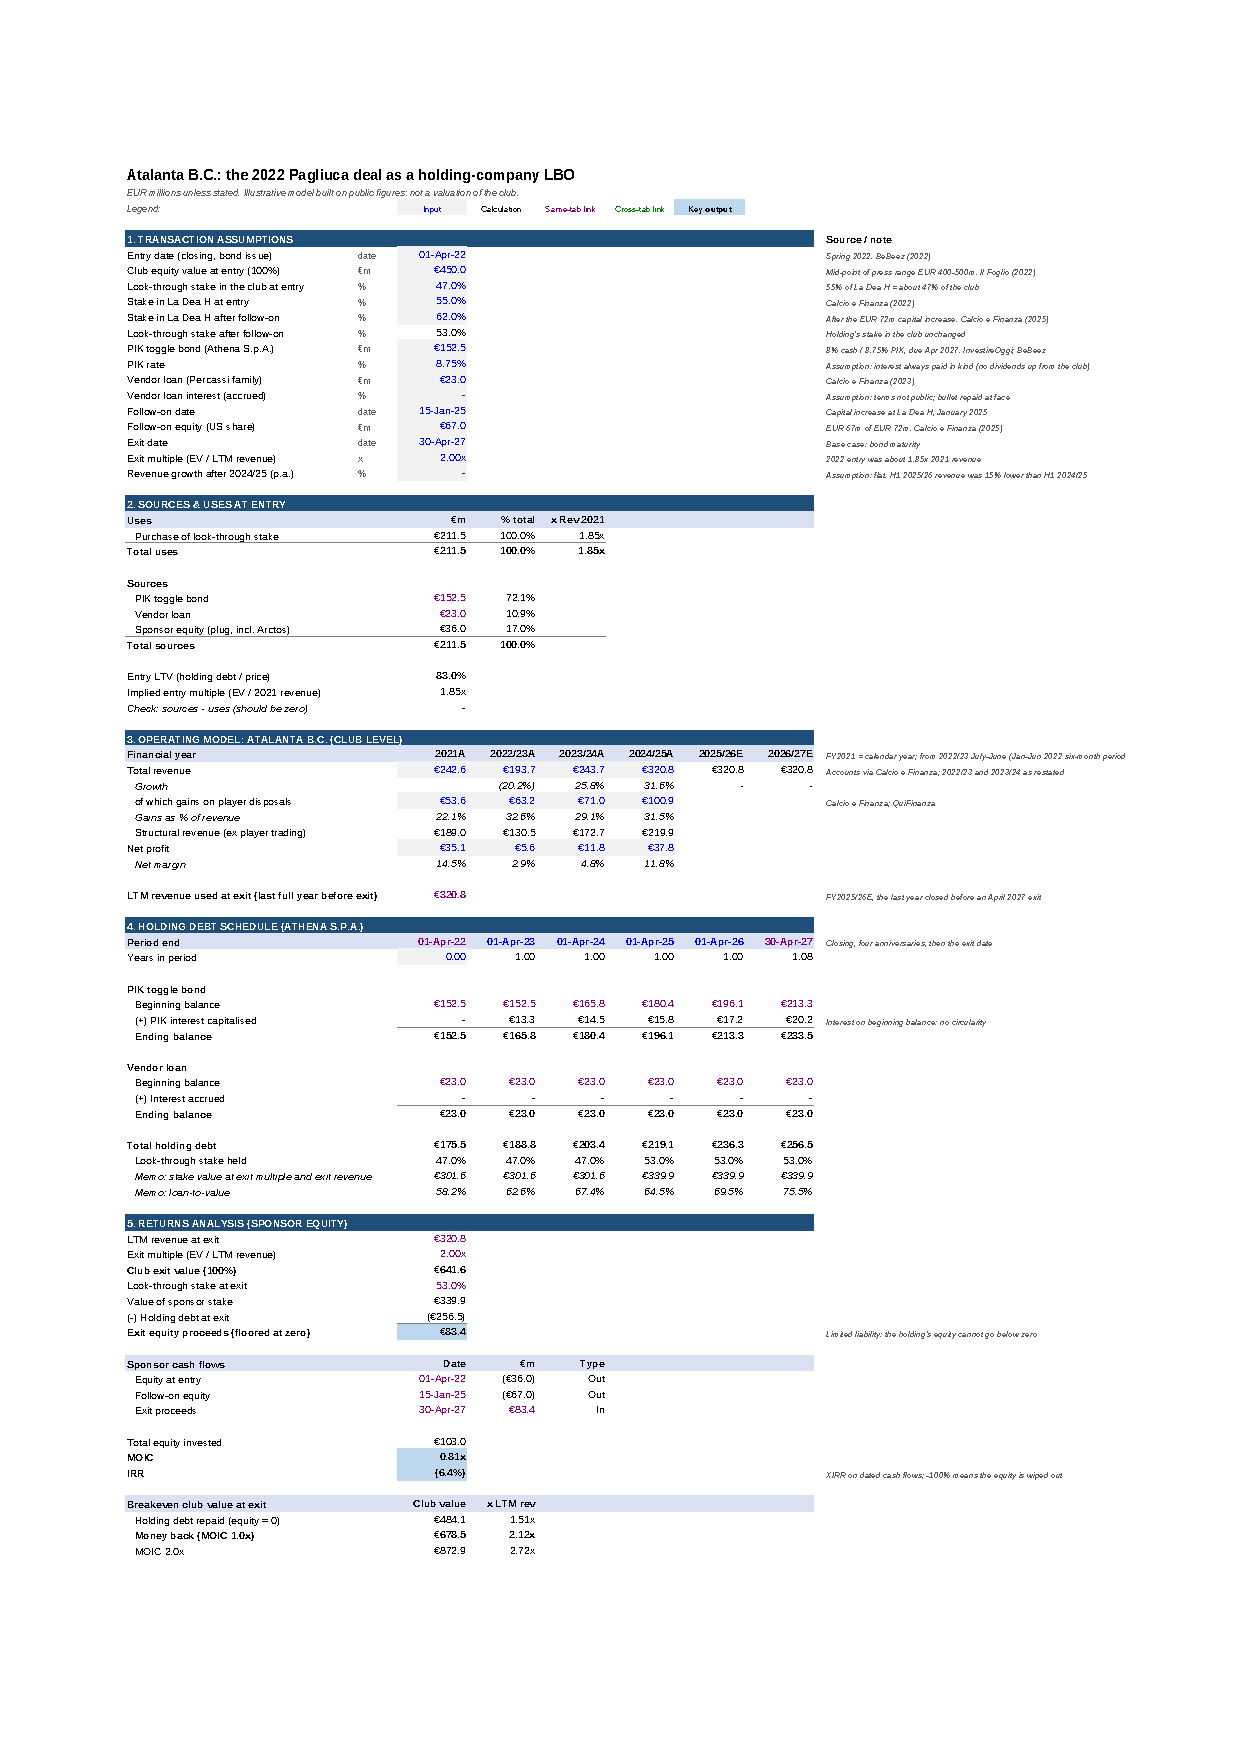
\includegraphics[width=\textwidth,trim=56 93 203 436,clip,page=1]{../model/atalanta_lbo_print.pdf}
\caption{The LBO model in Excel, part 2: the holding debt schedule (interest on the beginning balance, so no circular reference) and the returns analysis. Base case: exit at bond maturity at 2.0 times LTM revenue.}\label{fig:xlsx2}
\end{figure}

\begin{figure}[p]\centering
\includegraphics[width=\textwidth,trim=56 353 203 68,clip,page=2]{../model/atalanta_lbo_print.pdf}
\caption{The LBO model in Excel, part 3: four 5×5 sensitivity tables with the base case in the centre, the model checks and the debt against the value of the sponsor stake.}\label{fig:xlsx3}
\end{figure}

Some limits. Fees, the actual use of the PIK toggle, any dividends paid to the holding and the terms of the vendor loan are not public, and the exit is valued on revenue alone. The model is a way to see how the structure works, not an estimate of what the investors will earn.

\FloatBarrier
\section{After Gasperini}
Gasperini left in June 2025 after nine seasons \citep{ilpost_gasperini}. In twelve months the club changed coach three times: Juric in summer 2025, Palladino in November 2025 after Juric's dismissal (EUR~7.6m of termination costs), and Sarri in summer 2026. Even so, the first half of 2025/26 closed with EUR~27.1m of profit, and sales kept producing record gains (Table~\ref{tab:h1}).

\begin{table}[H]\centering\small
\caption{First half (July to December), EUR million. Source: \citet{cef_h1}.}\label{tab:h1}
\begin{tabular}{lrr}
\toprule
 & H1 2025/26 & H1 2024/25 \\
\midrule
Revenue & 175.8 & 207.1 \\
Gains on disposals & 57.3 & 85.9 \\
\quad of which Retegui and Ruggeri & 40.8 and 16.2 & \\
Net profit & 27.1 & 57.2 \\
Cash at the end of the period & 93.0 & 56.8 \\
\bottomrule
\end{tabular}
\end{table}

Profit halved compared with the record year but stayed positive, and the half-year does not yet include the sale of Lookman to Atlético Madrid in January 2026. The annual accounts to 30 June 2026 are not published yet; they usually come out in November.

\begin{figure}[htbp]\centering
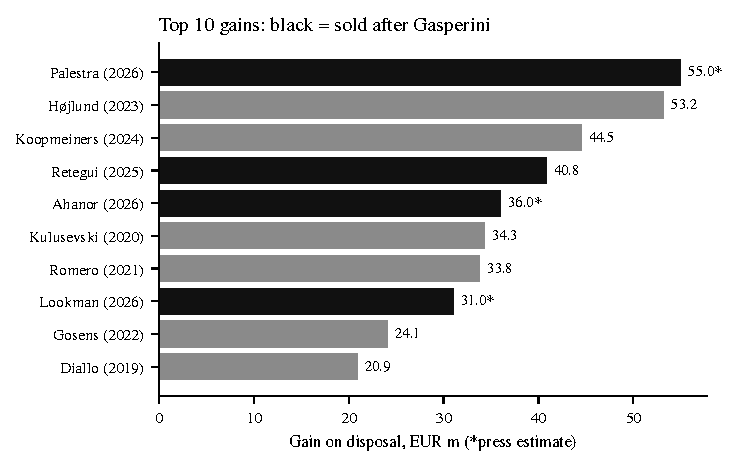
\includegraphics{../figures/fig6_top_sales.pdf}
\caption{The ten largest gains on disposal in the club's history, EUR million. Black: sold after Gasperini left. *Press estimates, not yet in the accounts. Sources: \citet{qf_plusvalenze,cef_palestra,cef_ahanor,cef_mercato2026}.}\label{fig:sales}
\end{figure}

Three of the five largest gains came after Gasperini (Figure~\ref{fig:sales}). Retegui and Lookman, though, were his signings: here the club is cashing in on the work of those years. The genuinely new cases are Palestra, from the academy, and Ahanor, bought from Genoa for EUR~16m in 2025 and sold to Chelsea for EUR~46.6m a year later \citep{cef_ahanor}. Season by season, gains went from EUR~63.2m (2022/23) to 71.0m (2023/24) and 100.9m (2024/25) \citep{cef_plus2024,cef_2425}, and 2025/26 started with 57.3m in the first half alone. Ederson, much discussed in May and June 2026, stayed at Atalanta. The mechanism works without the coach who made it famous; the full test will be Sarri's team.

\section{Risks}
I did not want this work to read as praise, so I listed what could break the model (Table~\ref{tab:risks}).

\begin{table}[H]\centering\small
\caption{Main risks of the model.}\label{tab:risks}
\begin{tabularx}{\textwidth}{P{2.8cm}LL}
\toprule
Risk & What the numbers say & What mitigates it \\
\midrule
Dependence on sales & Without sales, EBIT 2024/25 about EUR~−62m & Established academy and scouting network; Ahanor and Palestra in 2026 \\
Rising fixed costs & Personnel from EUR~84.4m (2022/23) to 127.4m (2024/25), +51\%; player amortisation from 48.9m to 71.2m in one year, +45\% & Wages still below the Serie A average relative to revenue \\
Revenue volatility & In 2022/23, without Europe, revenue of EUR~193.7m; H1 2025/26 revenue down 15\% & EUR~93m of cash; payables to clubs covered by receivables \\
Coaching continuity & Three coaches in a year; Juric's dismissal cost EUR~7.6m & Stable ownership and management since 2010 \\
Holding debt & EUR~152.5m bond maturing April 2027 & Debt outside the club; shareholders already recapitalised in 2025 \\
\bottomrule
\end{tabularx}
\end{table}

The more registrations the club buys, the more gains it needs later to cover their amortisation. That is the mechanism to watch in the next accounts. As a risk manager I would read the club as a portfolio with a high return and a concentrated exposure. The way to diversify is to grow the revenue that does not depend on the transfer market: commercial income and the stadium, together still below 17\% of turnover.

\section{Conclusion}
Atalanta shows that a Serie A club can be competitive and profitable, provided it treats selling players as its trade. It did so for ten years in a row, and the first season without Gasperini suggests that the mechanism did not depend on him alone.

I take two things from this work. First, financial statements have to be taken apart: once recurring revenue is separated from gains on disposals, the view on profitability changes, and the bottom line alone says little. Second, a model can work very well and still be fragile if it depends on a single engine. These are the questions I find most interesting in finance: what an asset is worth, how recurring a profit is, and where the risk is concentrated.

\medskip
\textit{Data and code: notebook, data files and charts at \href{https://github.com/ettoremancuso/atalanta-business-model}{github.com/ettoremancuso/atalanta-business-model}.}

\renewcommand{\refname}{References}
\begin{thebibliography}{99}\small\setlength{\itemsep}{2pt}
\bibitem[BeBeez(2022)]{bebeez} BeBeez (2022). Financing of the Atalanta acquisition. 19 May 2022. \url{https://bebeez.eu/2022/05/19/italys-private-debt-distressed-assets-and-npls-weekly-roundp-news-from-atalanta-carel-industries-iccrea-illimity-generalfinance-alia-servizi-ambientali-kervis-and-more/}
\bibitem[Calcio e Finanza(n.d.a)]{cef_1620} Calcio e Finanza (n.d.a). Atalanta, i conti 2016--2020. \url{https://www.calcioefinanza.it/?p=97846}
\bibitem[Calcio e Finanza(n.d.b)]{cef_2021} Calcio e Finanza (n.d.b). Atalanta, il bilancio 2021. \url{https://www.calcioefinanza.it/?p=97548}
\bibitem[Calcio e Finanza(2022)]{cef_pagliuca} Calcio e Finanza (2022). Pagliuca: rafforzare l'Atalanta. 17 May 2022. \url{https://www.calcioefinanza.it/2022/05/17/pagliuca-rafforzare-atalanta/}
\bibitem[Calcio e Finanza(n.d.c)]{cef_mercato2023} Calcio e Finanza (n.d.c). Atalanta, le cifre ufficiali del mercato 2023. \url{https://www.calcioefinanza.it/?p=137520}
\bibitem[Calcio e Finanza(2023)]{cef_pegno} Calcio e Finanza (2023). Atalanta, il bond e il pegno a Carlyle e Ares. 14 April 2023. \url{https://www.calcioefinanza.it/2023/04/14/atalanta-bond-pegno-carlyle-ares/}
\bibitem[Calcio e Finanza(n.d.d)]{cef_2324} Calcio e Finanza (n.d.d). Atalanta, il bilancio 2023/24. \url{https://www.calcioefinanza.it/?p=171049}
\bibitem[Calcio e Finanza(2024)]{cef_plus2024} Calcio e Finanza (2024). Atalanta, plusvalenze record nel 2024. 13 November 2024. \url{https://www.calcioefinanza.it/2024/11/13/atalanta-plusvalenze-2024-percassi/}
\bibitem[Calcio e Finanza(2025a)]{cef_seriea2324} Calcio e Finanza (2025a). Bilanci Serie A 2023/24: fatturato, costi e risultato netto. 25 January 2025. \url{https://www.calcioefinanza.it/2025/01/25/bilanci-serie-a-2024-fatturato-costi-risultato-netto-perdita/}
\bibitem[Calcio e Finanza(2025b)]{cef_aucap} Calcio e Finanza (2025b). Atalanta, nuovo socio USA e aumento di capitale. 8 January 2025. \url{https://www.calcioefinanza.it/2025/01/08/atalanta-nuovo-socio-usa-aumento-capitale/}
\bibitem[Calcio e Finanza(2025c)]{cef_2425} Calcio e Finanza (2025c). Atalanta, il bilancio 2025: ricavi, costi e utile. 20 November 2025. \url{https://www.calcioefinanza.it/2025/11/20/atalanta-bilancio-2025-ricavi-costi-utile/}
\bibitem[Calcio e Finanza(2026a)]{cef_seriea2425} Calcio e Finanza (2026a). Classifica bilanci Serie A 2024/25 per risultato netto. 2 February 2026. \url{https://www.calcioefinanza.it/2026/02/02/classifica-bilanci-serie-a-2024-2025-risultato-netto-utile/}
\bibitem[Calcio e Finanza(2026b)]{cef_h1} Calcio e Finanza (2026b). Atalanta, la semestrale 2025/26. 2 March 2026. \url{https://www.calcioefinanza.it/2026/03/02/atalanta-bilancio-semestrael-2025-2026-ricavi-costi/}
\bibitem[Calcio e Finanza(2026c)]{cef_bayern} Calcio e Finanza (2026c). Atalanta e Bayern Monaco a confronto: stipendi, bilanci, utili. 10 March 2026. \url{https://www.calcioefinanza.it/2026/03/10/atalanta-bayern-monaco-confronto-stipendi-bilanci-utili/}
\bibitem[Calcio e Finanza(2026d)]{cef_palestra} Calcio e Finanza (2026d). Palestra al Chelsea: la plusvalenza dell'Atalanta. 24 June 2026. \url{https://www.calcioefinanza.it/2026/06/24/palestra-plusvalenza-atalanta-cifre-chelsea/}
\bibitem[Calcio e Finanza(2026e)]{cef_ahanor} Calcio e Finanza (2026e). Ahanor al Chelsea: la plusvalenza dell'Atalanta. 27 August 2026. \url{https://www.calcioefinanza.it/2026/08/27/ahanor-plusvalenza-atalanta-chelsea/}
\bibitem[Calcio e Finanza(n.d.e)]{cef_mercato2026} Calcio e Finanza (n.d.e). Atalanta, il mercato estivo 2026. \url{https://www.calcioefinanza.it/?p=235855}
\bibitem[Calciomercato.com(n.d.)]{cm_koop} Calciomercato.com (n.d.). Koopmeiners dall'Atalanta alla Juventus: plusvalenza e percentuale all'AZ. \url{https://www.calciomercato.com/news/koopmeiners-dall-atalanta-alla-juventus-plusvalenza-e-percentuale-az-alkmaar-cifre-dettagli-66860}
\bibitem[Il Foglio(2022)]{ilfoglio} Il Foglio (2022). Il capolavoro di Percassi, che con l'Atalanta ha venduto un pezzo di cuore. 21 February 2022. \url{https://www.ilfoglio.it/economia/2022/02/21/news/il-capolavoro-di-percassi-che-con-latalanta-ha-venduto-un-pezzo-di-cuore--147231}
\bibitem[Il Giorno(n.d.)]{ilgiorno_stadio} Il Giorno (n.d.). Gewiss Stadium, i lavori e la presentazione di Percassi. \url{https://www.ilgiorno.it/bergamo/cronaca/stadio-gewiss-lavori-presentazione-percassi-988ebc82}
\bibitem[Il Post(2025)]{ilpost_gasperini} Il Post (2025). Gasperini è il nuovo allenatore della Roma. 6 June 2025. \url{https://www.ilpost.it/2025/06/06/gasperini-allenatore-roma-ufficiale/}
\bibitem[InvestireOggi(n.d.)]{investireoggi} InvestireOggi (n.d.). Bond Atalanta con maxi cedola all'8\%. \url{https://www.investireoggi.it/bond-atalanta-con-maxi-cedola-8-ecco-lobbligazione-della-dea/}
\bibitem[Italpress(n.d.)]{italpress_stadio} Italpress (n.d.). Il finanziamento per lo stadio dell'Atalanta. \url{https://www.italpress.com/?p=167266}
\bibitem[QuiFinanza(n.d.)]{qf_plusvalenze} QuiFinanza (n.d.). Atalanta, le plusvalenze dell'era Percassi. \url{https://quifinanza.it/sport-economy/atalanta-percassi-plusvalenze-valore/1005164/}
\end{thebibliography}
\end{document}
